%!TEX root = ../thesis.tex

\section{ニューラルネットワーク}
ニューラルネットワーク(Neural Network)は,人間の脳の神経回路に着想を得た計算モデルであり,機械学習で重要な役割を担う.このモデルは,大量のデータから学習し,パターン認識や予測などの複雑なタスクを遂行できる点が特徴である.以下に基本的な構造を示す.

% ニューラルネットワークは,多数のノード(ニューロン)が層状に接続された構造を持つ.各ノードは入力信号を受け取り,重み付けを行い,活性化関数を適用することで出力信号を生成する.

\begin{itemize}
     \item \textbf{入力層(Input Layer)}\\
     入力データを受け取る層であり,各ノードが入力データの各特徴量に対応する.
     \item \textbf{隠れ層(Hidden Layer)}\\
     入力層と出力層の間に位置する層である.複数の隠れ層を設けることで,複雑な非線形関係をモデル化でき,より高度な特徴表現の獲得が可能となる.
     \item \textbf{出力層(Output Layer)}\\
     ネットワークの最終的な出力を生成する層である.
\end{itemize}

\figref{Fig:neural-network}のように,各層のノードは次の層のノードと相互に接続され,接続には重みが割り当てられている.学習の過程では,誤差逆伝播などの最適化手法を用いてこれらの重みを調整し,ネットワークが目的のタスクを精度良く実行できるように最適化される.
多層構造を持つことで複雑なパターンや特徴を学習し,従来では困難であった高精度な予測を実現した学習手法を深層学習と呼ぶ.深層学習は,画像認識や自然言語処理,音声認識など幅広い分野で活用されており,YOLO(You Only Look Once)\cite{redmon2016you-yolo}やChatGPT\cite{radford2018improving-gpt, radford2019language-gpt,brown2020language-gpt}といった成功例が多数存在し,高い性能が評価されている.

% \vspace{-30pt}

\begin{figure}[H]
     \centering
    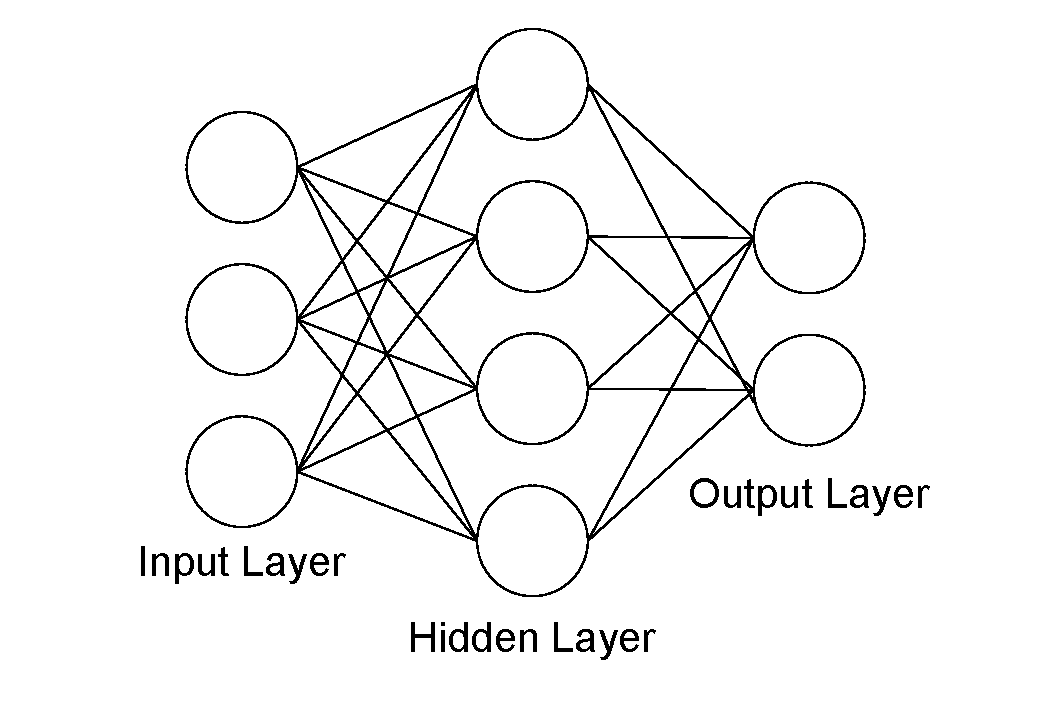
\includegraphics[keepaspectratio, scale=0.37]
         {images/neural-network.pdf}
    \caption{Neural network}
    \label{Fig:neural-network}
\end{figure}   

\newpage
